\documentclass[fadttsterUserGuide_use]{subfiles}

\begin{document}
	\section{Matlab script generation}
	The \textit{Matlab script generation} is the reason why FADTTSter was originally developed. The idea was to ``hide'' every technical aspect for the writing of the Matlab script --- used to generate the statistical data --- with a user-friendly GUI interface. Subsequently, the tool was implemented with some options (subjects management, quality control, profile cropping, etc). Then FADTTSter was made available as a command line only based tool.
	
	\subsection{FADTTSter --- GUI interface}
	The \textit{Matlab script generation} regroups the first three tabs of FADTTSter: \textit{Inputs}, \textit{Subjects} and \textit{Execution}.
	\vfill
	\begin{figure}[H]
		\makebox[\linewidth][c]
		{
			\centering
	    	\begin{subfigure}{0.5\textwidth}
				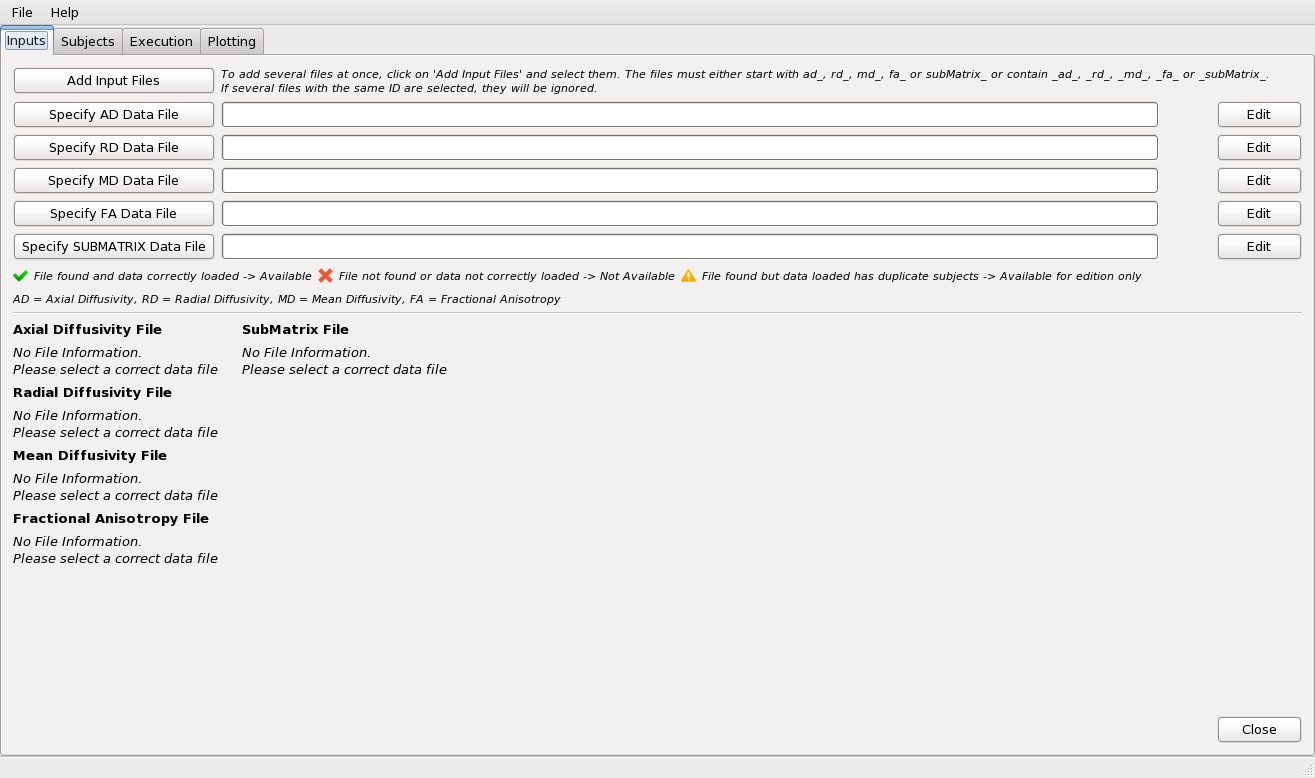
\includegraphics[width=\textwidth]{inputTab_blank}
   	    	 	\caption{Inputs tab}
   	     		\label{subfig:inputsTab_blank}
			\end{subfigure}
			\begin{subfigure}{0.5\textwidth}
        		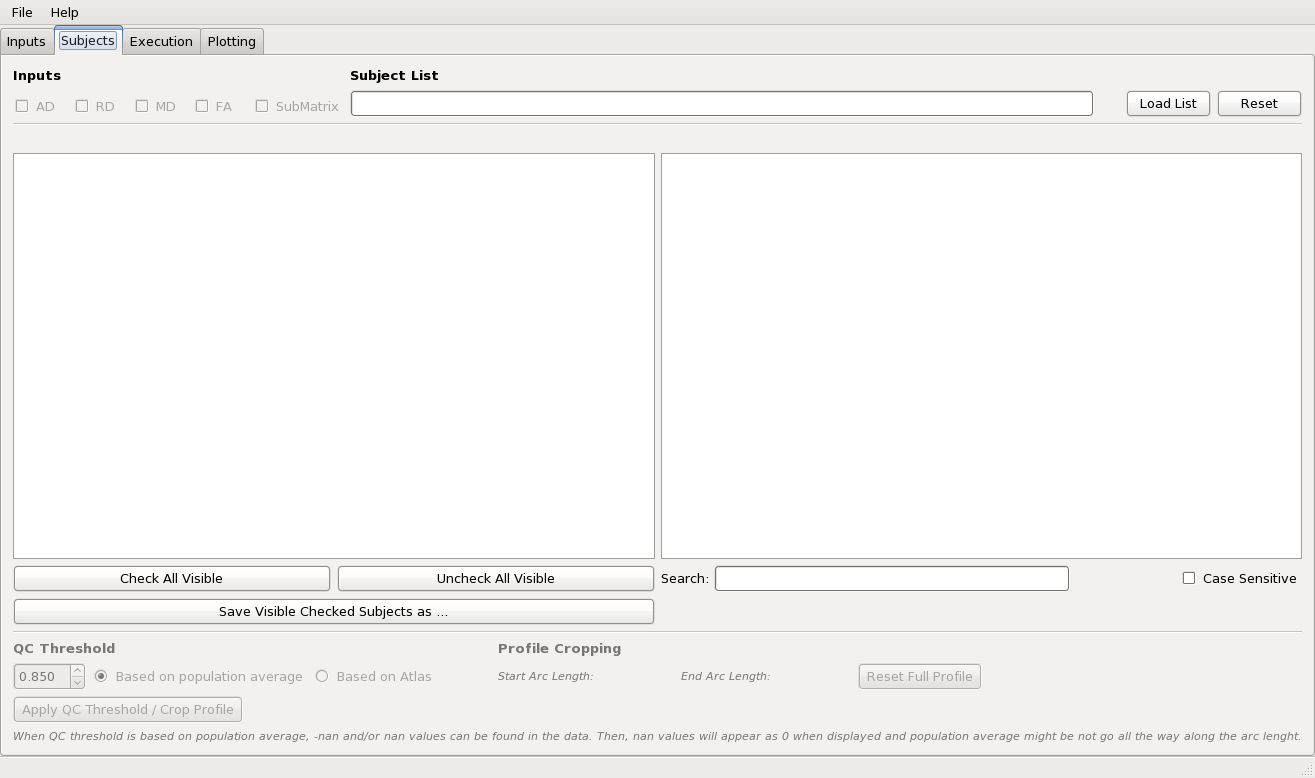
\includegraphics[width=\textwidth]{subjectsTab_blank}
        		\caption{Subjects tab}
        		\label{subfig:subjectsTab_blank}
    		\end{subfigure}
    		\begin{subfigure}{0.5\textwidth}
        		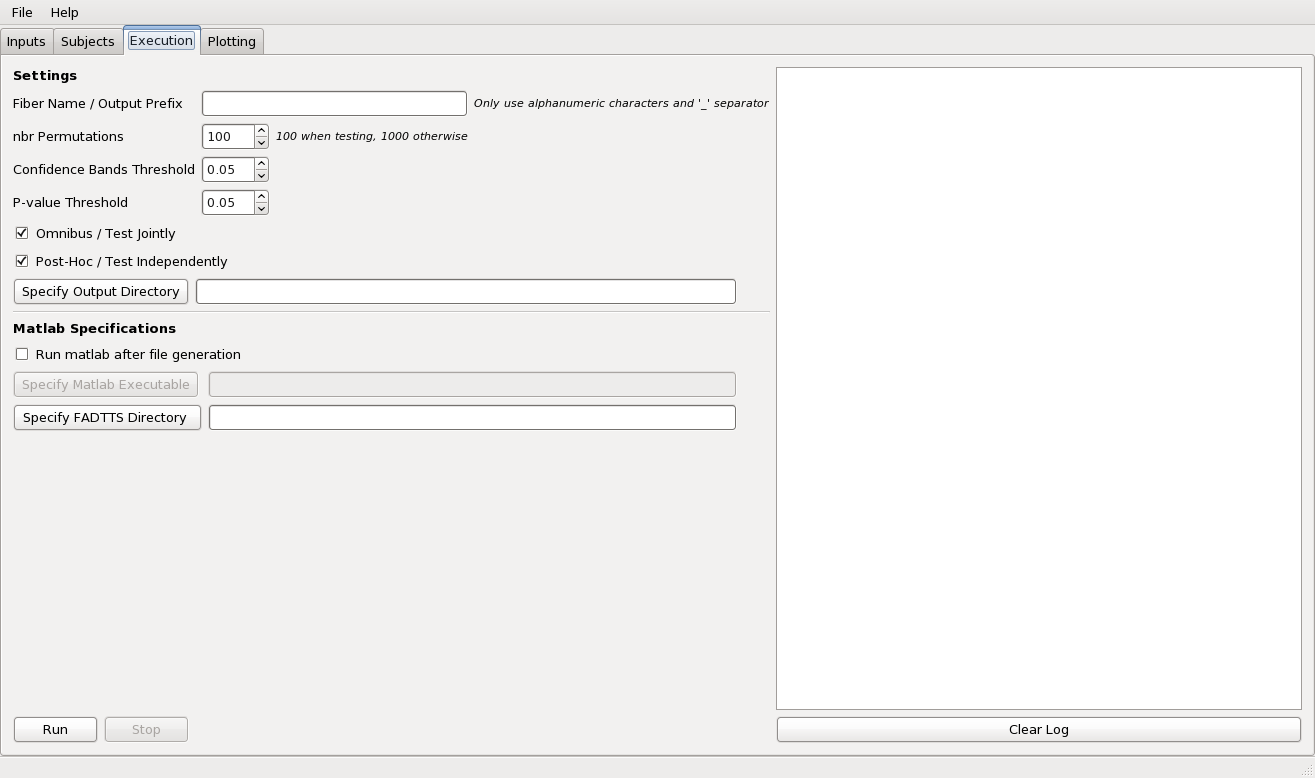
\includegraphics[width=\textwidth]{executionTab_blank}
        		\caption{Execution tab}
        		\label{subfig:executionTab_blank}
    		\end{subfigure}
    	}
    	\caption{FADTTSter tabs used for \textit{Matlab script generation}}
    	\label{fig:matlabScriptGeneration_Tabs}
	\end{figure}
	\vfill
	\vfill
	\newpage
	
	\subsubsection{Inputs tab}
	\begin{figure}[H]
  		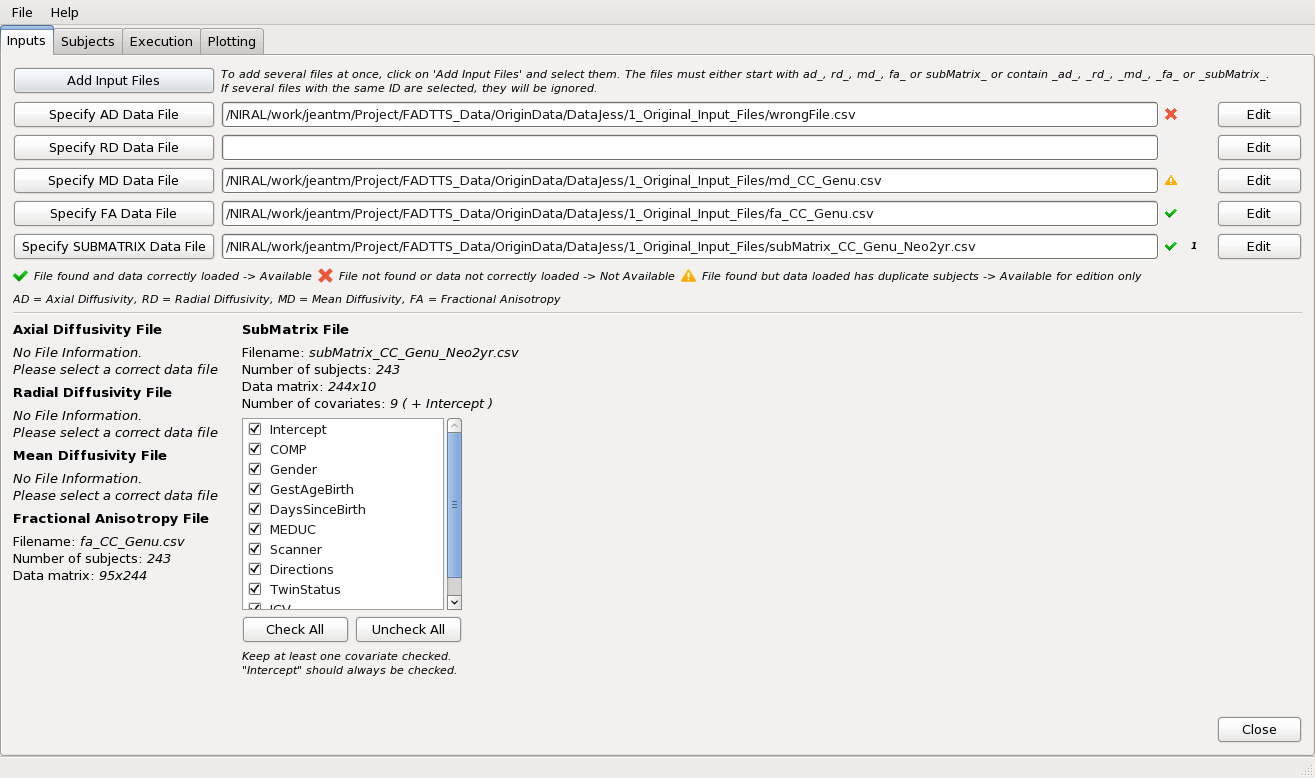
\includegraphics[width=1.36\textwidth,center]{inputTab_filed}
  		\caption{Inputs tab}
    	\label{fig:inputsTab_filed}
	\end{figure}
	The \textit{Inputs} tab allows the user to set and edit the diffusion property files and the covariates file and set the covariates for the ongoing study.
	\vfill
	\newpage
	
	\paragraph{Add input files}
	\begin{itemize}
		\item \textbf{Add several files at once:}
		\begin{enumerate}
			\item Click on ``Add Input Files''
			\begin{figure}[H]
  				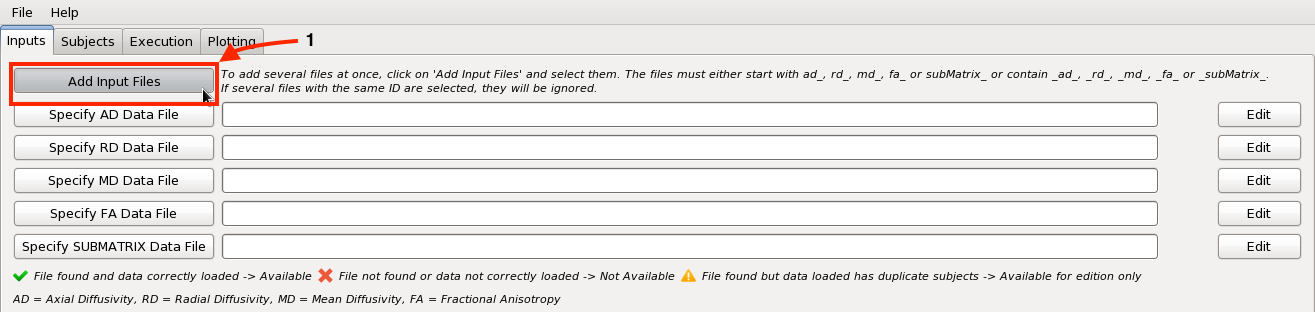
\includegraphics[width=1.0\textwidth,center]{addMultipleFiles1}
  				\caption{Adding input files}
    			\label{fig:addInputFiles_pushButton}
			\end{figure}
			\item In the pop-up window displayed, browse to the folder containing the files you want to add
			\item Select them
			\item Click on ``Open''
			\begin{figure}[H]
  				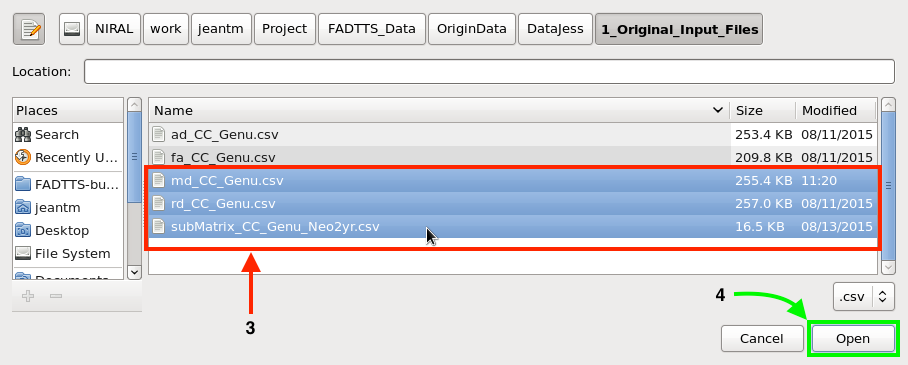
\includegraphics[width=1.0\textwidth,center]{addMultipleFiles2}
  				\caption{Pop-up window displayed to set multiple input files at once}
    			\label{fig:addMultipleInputFiles_popUp}
			\end{figure}
		\end{enumerate}
	\end{itemize}
	\subparagraph{\textbf{Note:}}
	\begin{itemize}
		\item[--] The default format for the input files is \textit{.csv}.
		\item[--] The selection is not case sensitive.
	\end{itemize}	 
	\subparagraph{\textbf{WARNING:}}
	\begin{itemize}
		\item[--] Selected files must either start with \textit{ID}\_ or contain \_\textit{ID}\_
			\newline
			(\textit{ID} being \textit{AD}, \textit{RD}, \textit{MD}, \textit{FA} or \textit{SUBMATRIX})
			\vfill
			\newpage	
			
		\item[--] Selected files with the same \textit{ID} are ignored.
			\newline
			(e.g. If you select the following files the files: \textit{my\_ad\_file1.csv}, \textit{AD\_myfile2.csv}, \textit{my\_FA\_file.csv} and \textit{mySubmatrix\_file.csv}, only \textit{my\_FA\_file.csv} and \textit{mySubmatrix\_file.csv} will be added to the ongoing study.)
	\end{itemize}
	\begin{itemize}
		\item \textbf{Add one file:}
		\begin{enumerate}
			\item Click on ``Specify \textit{ID} Data File''
			\begin{figure}[H]
  				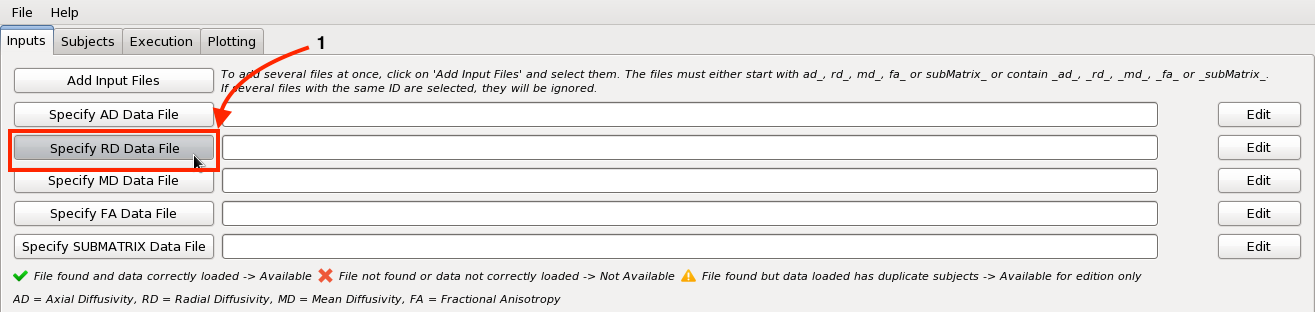
\includegraphics[width=1.0\textwidth,center]{addFile1}
  				\caption{Adding one file using ``Specify Data File'' push button}
    			\label{fig:specifyDataFile_pushButton}
			\end{figure}
			\item In the pop-up window displayed, browse to the folder containing the file you want to add
			\item Select it
			\item Click on ``Open'' or double click on the file
		\end{enumerate}	
			Or
		\begin{itemize}
			\item[] Give the absolute path to the file you want to add
			\begin{figure}[H]
  				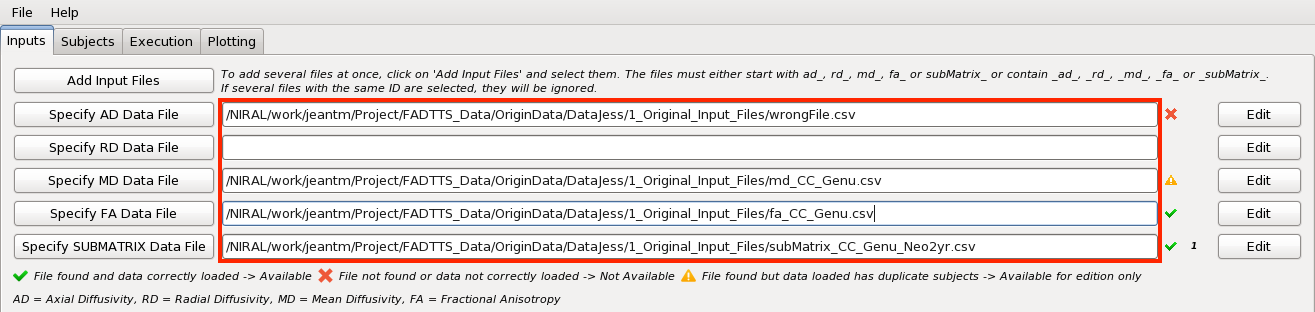
\includegraphics[width=1.0\textwidth,center]{addFile3}
  				\caption{Adding one file specifying the absolute path}
    			\label{fig:specifyDataFile_absolutePath}
			\end{figure}
		\end{itemize}
	\end{itemize}
	\subparagraph{\textbf{Note:}} Here, file name does not matter.
	\vfill
	\newpage
	
	\begin{itemize}
		\item \textbf{File status and file information:}
		\begin{figure}[H]
  			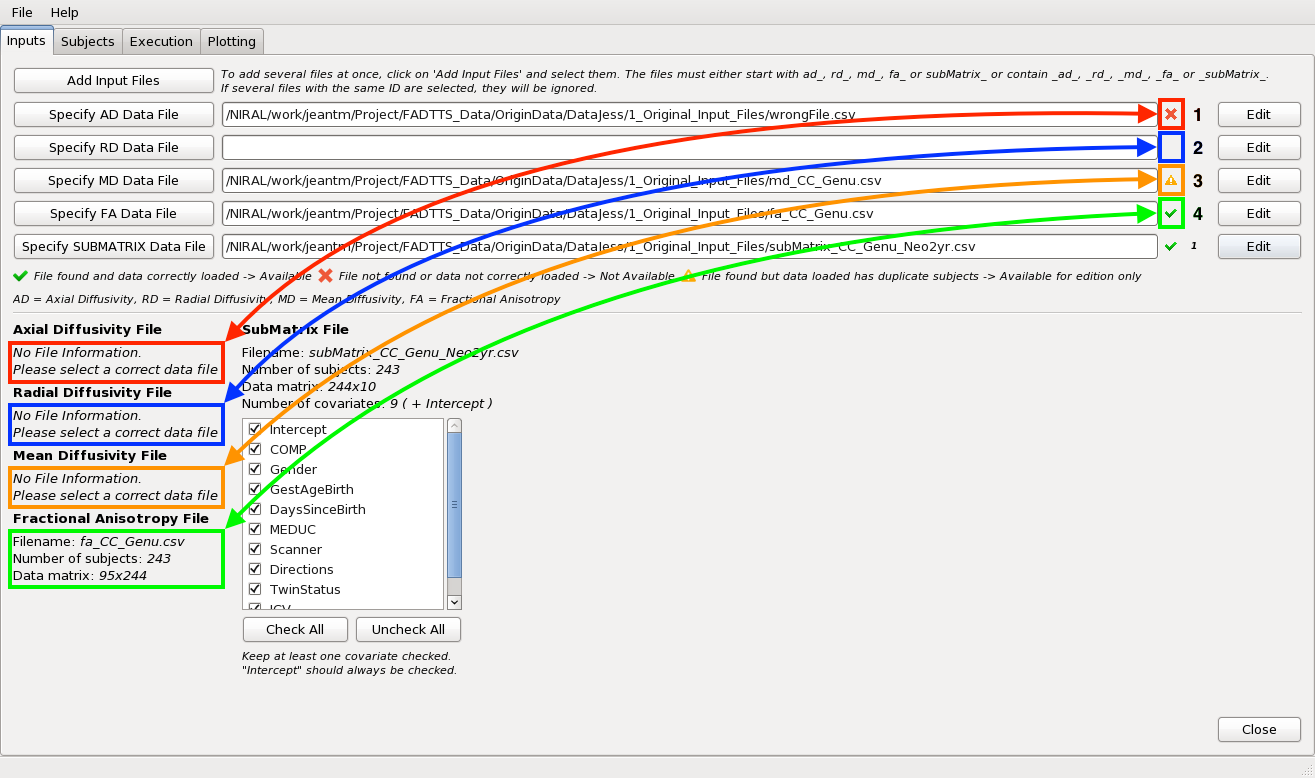
\includegraphics[width=1.0\textwidth,center]{fileStatusInformation}
  			\caption{File status and file information after adding an input file}
    		\label{fig:fileStatus}
		\end{figure}
		\begin{itemize}
			\item File not found or data not correctly loaded\textrightarrow Ignored (1)	
			\item File not provided (2)
			\item File found but data loaded has duplicate subjects\textrightarrow Available for edition only (2)
			\item File found and data correctly loaded\textrightarrow Available for the ongoing\newline study (4)
		\end{itemize}
	\end{itemize}
	The information provided contains:
	\begin{itemize}
			\item[--] The file name		
			\item[--] The number of subjects found
			\item[--] The size of the data matrix
	\end{itemize}
	In addition, for the covariates file, we have:
	\begin{itemize}
			\item[--] The number of covariates found and their names
			\item[--] The position of the column featuring the subjects
	\end{itemize}
	\subparagraph{\textbf{Note:}} All files must have the same data size. In other words, if an \textit{FA}, a \textit{RD} and a \textit{SubMatrix} file of respective data matrix size $M_{\textit{FA}}\times N_{\textit{FA}}$,  $M_{\textit{RD}}\times N_{\textit{RD}}$ and $M_{\textit{SubMatrix}}\times N_{\textit{SubMatrix}}$, then we must have $M_{\textit{FA}} = M_{\textit{RD}} = N_{\textit{SubMatrix}}$.
	\vfill
	\newpage
	
	\paragraph{Edit input files}
	The edition modifies the data loaded within the GUI but never the original data files.
	\begin{itemize}
		\item \textbf{Start edition:}
		\begin{enumerate}
			\item Click on ``Edit''
			\begin{figure}[H]
  				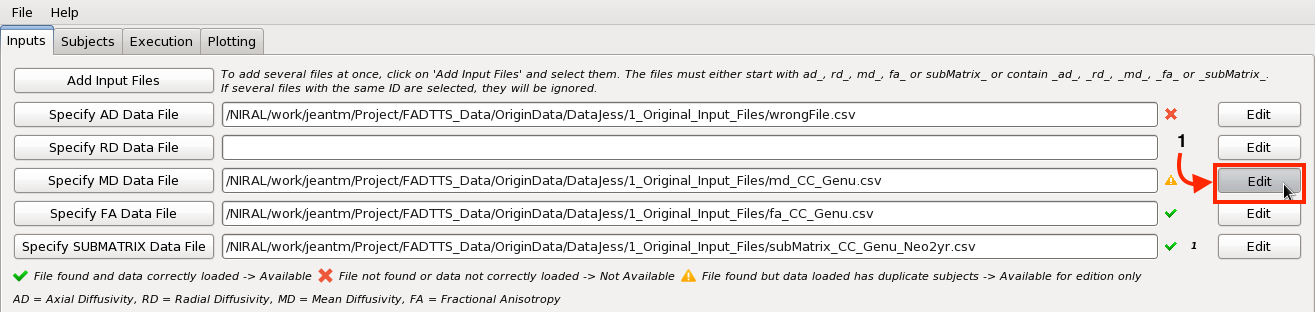
\includegraphics[width=1.0\textwidth,center]{editFile}
  				\caption{Editing an input file}
    			\label{fig:edit_pushButton}
			\end{figure}
			\begin{figure}[H]
  				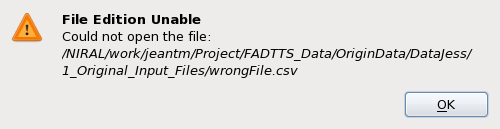
\includegraphics[width=0.7\textwidth,center]{popup_edit_wrongFile}
  				\caption{Pop-up window displayed when file edition is unavailable (i.e. no data has been loaded (file not provided or not found)}
    			\label{fig:warningPopUp_edition}
    		\end{figure}
			\item Start the file edition
			\begin{figure}[H]
				\makebox[\linewidth][c]
				{
					\centering
	    			\begin{subfigure}{0.7\textwidth}
						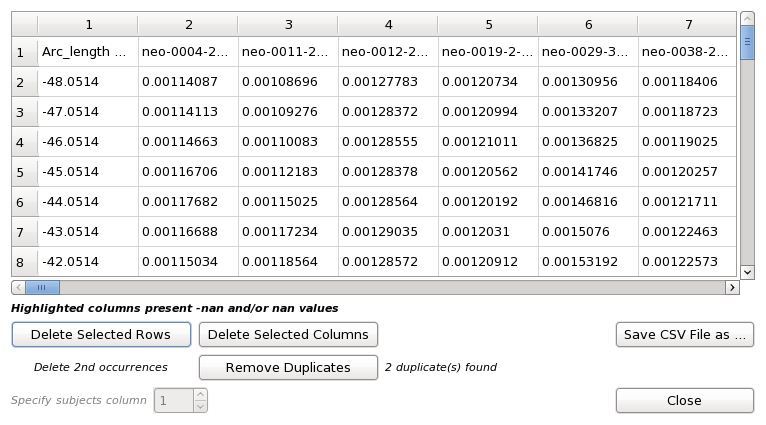
\includegraphics[width=\textwidth]{edit_diffusionFile}
   	    	 			\caption{Edition window displayed for a diffusion property file}
   	     				\label{subfig:editionWindow_diffusionPropertyFile}
					\end{subfigure}
					\begin{subfigure}{0.7\textwidth}
        				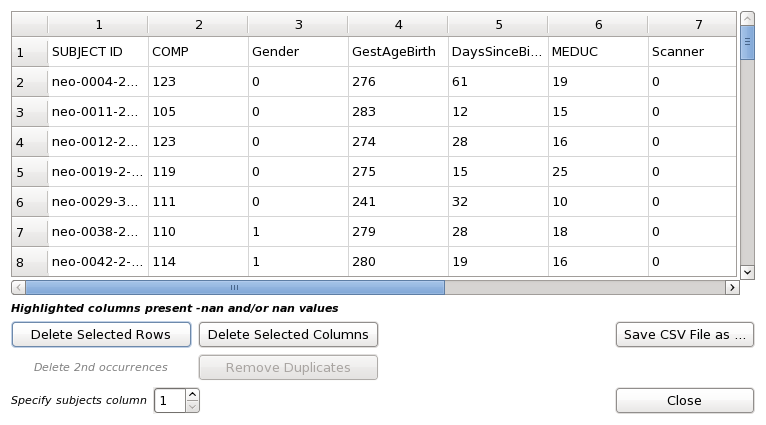
\includegraphics[width=\textwidth]{edit_covariatesFile}
        				\caption{Edition window displayed for a covariates file}
        				\label{subfig:editionWindow_covariatesFile}
    				\end{subfigure}
    			}
				\caption{Edition windows available depending on the input file provided}
    			\label{fig:editionWindow_covariatesFile}
			\end{figure}
		\end{enumerate}
	\end{itemize}
	\vfill
	\newpage
	
	\begin{itemize}
		\item \textbf{Delete column(s)/row(s):}
		\begin{enumerate}
			\item Select colomn(s)/row(s) to delete
			\item Click on ``Delete colomn(s)''/``Delete row(s)''
			\begin{figure}[H]
  				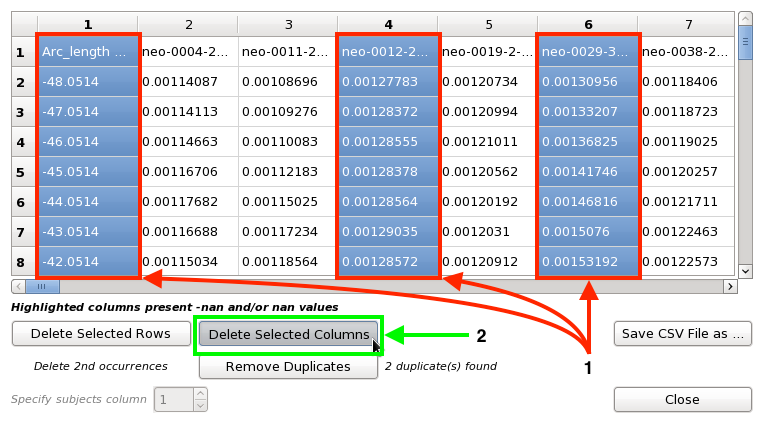
\includegraphics[width=0.95\textwidth,center]{deleteColumns}
  				\caption{Deleting columns}
    			\label{fig:editionWindow_deleteColumnsRows}
			\end{figure}
		\end{enumerate}
	\end{itemize}
	\begin{itemize}
		\item \textbf{Remove duplicates:}
		\begin{itemize}
			\item Click on ``Remove Duplicates''
			\begin{figure}[H]
  				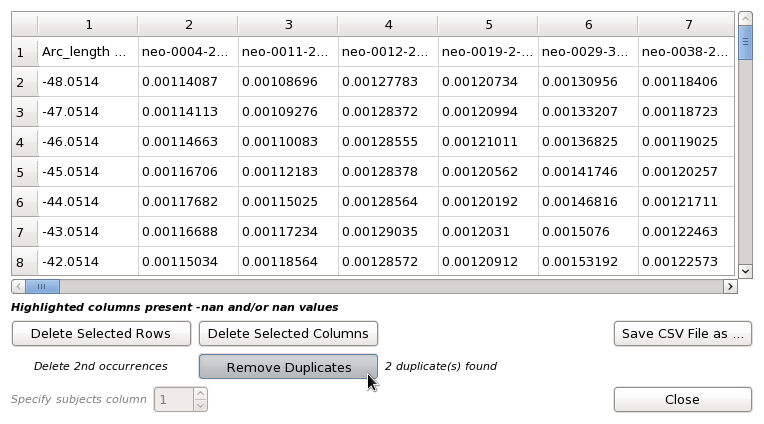
\includegraphics[width=0.9\textwidth,center]{removeDuplicates}
  				\caption{Removing duplicates from data file}
    			\label{fig:editionWindow_removeDuplicates}
			\end{figure}
		\end{itemize}
	\end{itemize}
	\subparagraph{\textbf{Note:}} Only second occurrences are deleted. Once applied, you cannot go back except by closing the editing window.
	\vfill
	\newpage
	
	\begin{itemize}
		\item \textbf{\textit{nan} values (FA file only):}
	\end{itemize}
		Some data can be set as \textit{nan} instead of a number. Should that be the case, the columns where at least one \textit{nan} value is found are highlight in a beautiful Carolina blue. It is the responsability of the user to keep the data.
	\begin{figure}[H]
  		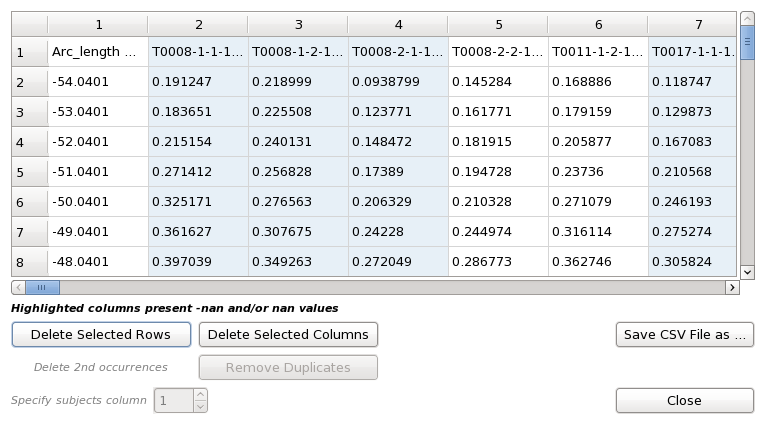
\includegraphics[width=0.9\textwidth,center]{edit_FAnan}
  		\caption{Nan values found in an FA file}
    	\label{fig:editionWindow_nanValues}
	\end{figure}
	\begin{itemize}
		\item \textbf{Change subjet column ID (covariates file only):}
		\begin{itemize}
			\item Set subjects column ID to the column where subjects are displayed
			\begin{figure}[H]
  				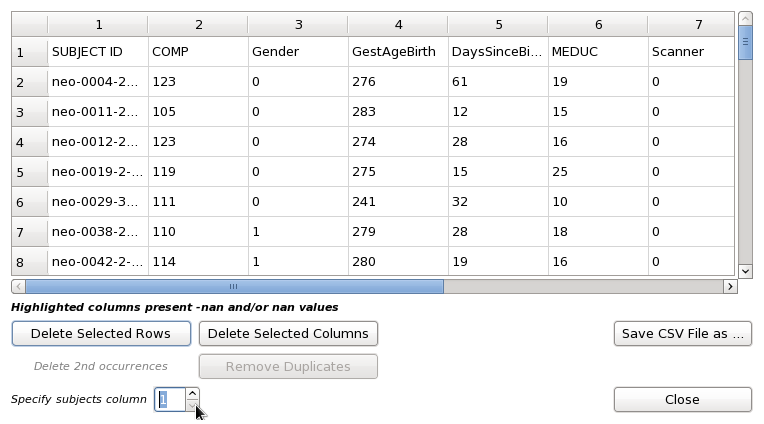
\includegraphics[width=0.9\textwidth,center]{subjectColumnID}
  				\caption{Setting column ID}
    			\label{fig:editionWindow_setColumnID}
			\end{figure}
		\end{itemize}
	\end{itemize}
	\subparagraph{\textbf{Note:}} Usually, the subjects are in the first column. If so, this feature should not be used.	
	\vfill
	\newpage
	
	\begin{itemize}
		\item \textbf{Save modifications:}
		\begin{enumerate}
			\item Click on ``Save CSV File as \ldots''
			\begin{figure}[H]
  				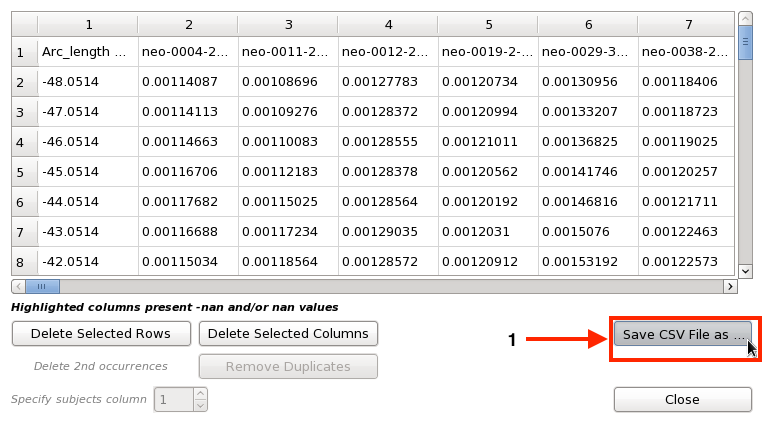
\includegraphics[width=1.0\textwidth,center]{saveModifications}
  				\caption{Save modifications after file edition}
    			\label{fig:saveModifications}
			\end{figure}
			\item In the pop-up window displayed, browse to the folder where you want to save your modification
			\item Rename the file if needed
			\item Click on ``Save''
		\end{enumerate}
	\end{itemize}
	\subparagraph{\textbf{Note:}}
	\begin{itemize}
		\item[--] Make sure to save the file as a \textit{.csv}
		\item[--] If modifications are made AND saved, the path to the input file is automatically updated.
		\item[--] If you close the edition window after making some modifications but without having saved them, the following pop-up will be displayed.
	\end{itemize}
	\begin{figure}[H]
  		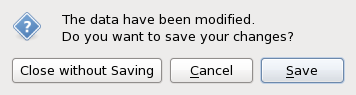
\includegraphics[width=0.5\textwidth,center]{closingEdition}
  		\caption{Closing pop-up displayed after modifications not saved}
    	\label{fig:editionWindow_closingPopUp}
	\end{figure}
	\vfill
	\newpage
	
	In that case you can:
	\begin{itemize}
		\setlength\itemindent{25pt}
		\item[--] \textit{Save} your modifications (cf previous point)
		\item[--] \textit{Discard} your modifications and go back to the main window with your data unchanged
		\item[--] \textit{Cancel} your decision and go back to the edition window
	\end{itemize}
	\subparagraph{\textbf{Note:}} As long as you do not write over the original file, it will remain unmodified, even if modification are applied.
	
	
	\paragraph{Select covariates}
	(Available only if a correct covariates file has been loaded)
	\begin{itemize}
		\item[--] Click on a covariate to select/unselect it individually
		\item[--] Click on ``Check All''/``Uncheck All'' to select/unselect all covariates
		\begin{figure}[H]
  			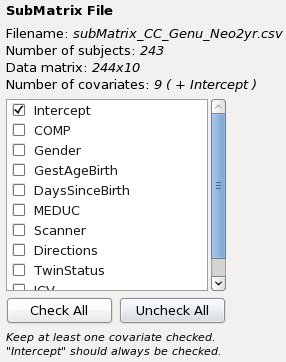
\includegraphics[width=0.35\textwidth,center]{allCovariatesUnselected}
  			\caption{Toggle the covariates to add them to or remove them from the study}
    		\label{fig:covariatesSelection}
		\end{figure}
	\end{itemize}
	\subparagraph{\textbf{WARNING:}} \textit{Intercept} should always be selected.
	\subparagraph{\textbf{Note:}}``Uncheck All'' will unselect all covariates but the \textit{Intercept}.
	\begin{figure}[H]
  		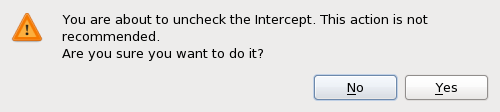
\includegraphics[width=0.75\textwidth,center]{warningUnselectiongIntercept}
  		\caption{Unselecting the \textit{Intercept} will result in displaying a warning pop-up}
    	\label{fig:unselectIntercept}
	\end{figure}
	\vfill
	\newpage
	
	\subsubsection{Subjects tab}
	\begin{figure}[H]
  		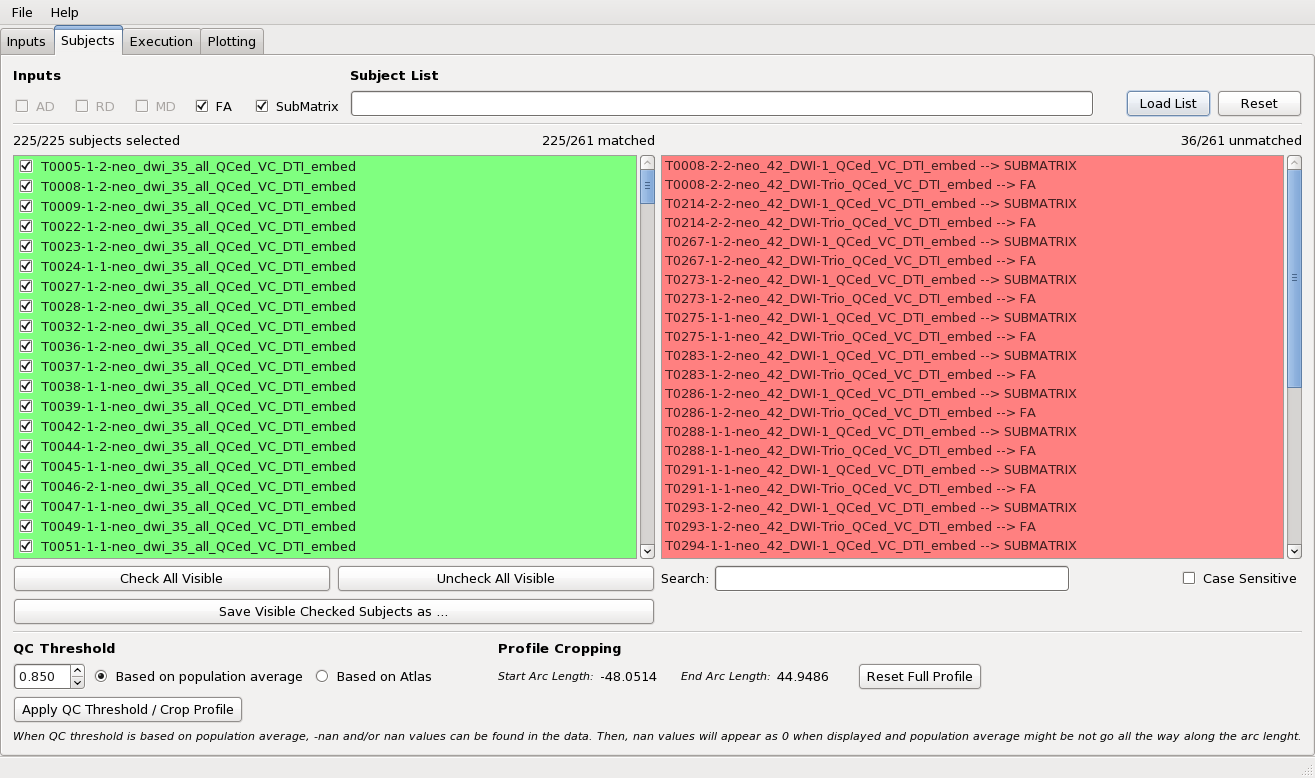
\includegraphics[width=1.36\textwidth,center]{subjectsTab_filed}
  		\caption{Subjects tab}
    	\label{fig:subjectsTab_blank}
	\end{figure}
	The \textit{Subjects} tab allows the user to manage the subjects of the ongoing study. They can be added to/removed from the study individually or after setting a quality control (QC) threshold. Through this tab, the user can also crop the profile.
	\vfill
	\newpage

	\paragraph{Add subjects}	
	\begin{itemize}
		\item \textbf{From input files:}
		\begin{itemize}
			\item Select the \textit{ID} (\textit{AD}, \textit{MD}, \textit{RD}, \textit{FA} or \textit{SUBMATRIX}) of the input file which subject list you want to add.
		\end{itemize}
		\begin{figure}[H]
  			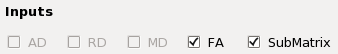
\includegraphics[width=0.50\textwidth,center]{addSubjects}
  			\caption{Adding subjects from input files}
    		\label{fig:addSubjectsFromFiles}
		\end{figure}
	\end{itemize}
	\subparagraph{\textbf{Note:}} Every input file provided in the \textit{Inputs} tab is linked to a single diffusion property file (\textit{AD}, \textit{MD}, \textit{RD} or \textit{FA}) or to the covariates file (\textit{SUBMATRIX}). Everytime an input file is correctly added and loaded, its selection is enabled in the \textit{Subjects} tab.
	\begin{itemize}
		\item \textbf{From external subject list:}
		\begin{enumerate}
			\item Click on ``Load List''
			\begin{figure}[H]
  				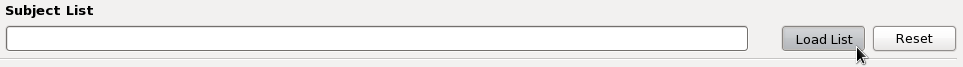
\includegraphics[width=1.25\textwidth,center]{loadExternalSubjectList}
  				\caption{Adding a subjects from an external subject list}
    			\label{fig:addSubjectsFromExternalList}
			\end{figure}
			\item In the pop-up window displayed, browse to the folder containing the external subject list you want to add
			\item Select it
			\item Click on ``Open'' or double click on it
		\end{enumerate}
	\end{itemize}
	\subparagraph{\textbf{Note:}} Default format for the external subject list is \textit{.txt}.
	
	
	\paragraph{Manage subjects}
	\begin{itemize}
		\item \textbf{Display:}
		\newline
		Once the subjects have been added to the study from input files and/or an external subject list, they are sorted in two categories and displayed. The \textit{matched subjects} are the subjects that have been found in all the subject lists provided. The \textit{unmatched subjects} are the ones missing in at least one of the subject lists provided. Subjects within the \textit{unmatched} group are automatically excluded from the study. Only the ones from the \textit{matched} group can be added to the study at the user's convenience.	
		\vfill
		\newpage
		
		\begin{figure}[H]
  			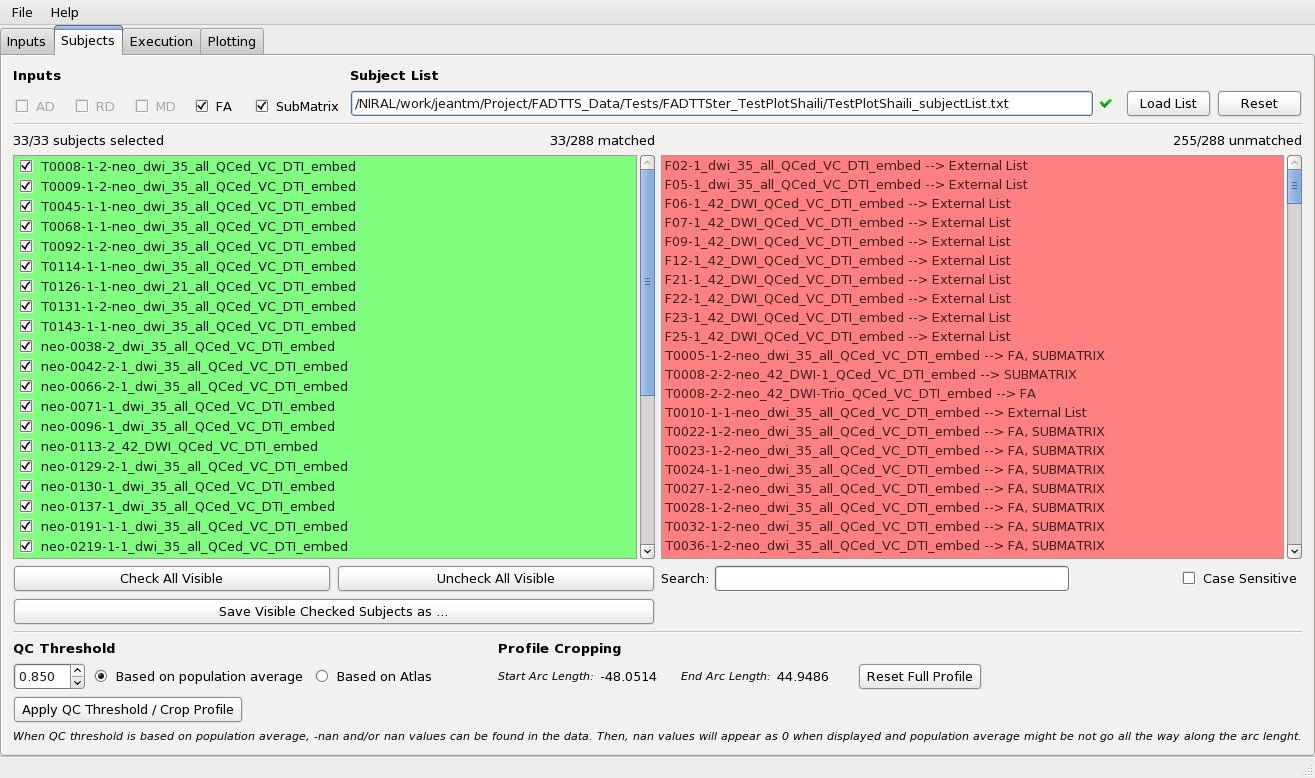
\includegraphics[width=1.0\textwidth,center]{displaySubjects}
  			\caption{Subjects displayed regarding their occurrences in all subject lists provided}
    		\label{fig:displaySubjects}
		\end{figure}
	\end{itemize}
	\subparagraph{\textbf{Note:}}
	\begin{itemize}
		\item[--] In the \textit{unmatched} window, subjects are displayed as follow:
			\newline
			\centerline{\textit{subject\_name}\textrightarrow \textit{occurence 1}, \textit{occurence 2}, etc}
			\newline
			(e.g. Sujects are added from an \textit{AD}, \textit{RD} and \textit{FA} file and an external subject list. If ``Marcus\_Paige'' is found only in the \textit{AD} file subject lists and in the external subject list, then it will be displayed in the \textit{unmatched} window as: \textit{Marcus\_Paige\textrightarrow AD, external subject list})
		\item[--] On top of both display windows, information is provided about:
		\begin{itemize}
			\setlength\itemindent{25pt}
			\item[-] the number of subjects selected (\textit{nbr of subjects selected}/\textit{total nbr of} matched \textit{sujects})
			\item[-] the number of \textit{matched} subjects (\textit{nbr of} matched \textit{subjects}/\textit{total nbr of subjects}
			\item[-] the number of \textit{unmatched} subjects (\textit{nbr of} unmatched \textit{subjects}/\textit{total nbr of subjects}
		\end{itemize}
	\end{itemize}
	\begin{figure}[H]
  		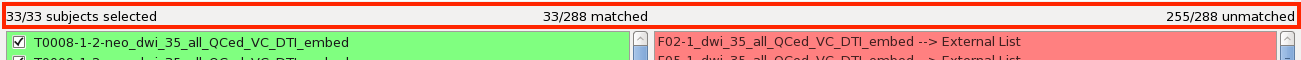
\includegraphics[width=1.25\textwidth,center]{displaySubjects2}
  		\caption{Information provided regarding the subjects displayed}
    	\label{fig:subjectsInformation}
	\end{figure}
	\vfill
	\newpage
	
	\begin{itemize}
		\item \textbf{Select subject:}
		\begin{itemize}
			\item Click on the subjects you want to add/remove
		\end{itemize}
		Or
		\begin{itemize}
			\item Click on ``Check All Visible''/``Uncheck All Visible'' to select/unselect all \emph{visible subjects}
			\begin{figure}[H]
  				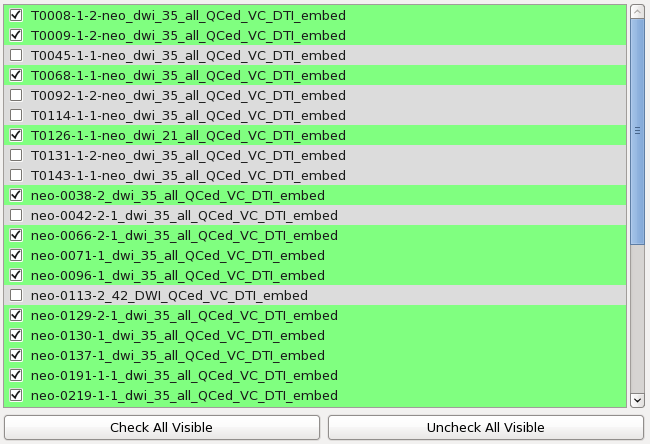
\includegraphics[width=0.6\textwidth,center]{addRemoveSubjects}
  				\caption{Selecting/unselecting a specific subject by clicking on it}
    			\label{fig:addRemoveSubjects}
			\end{figure}
		\end{itemize}
	\end{itemize}
	\begin{itemize}
		\item \textbf{Save subject list:}
		\begin{enumerate}
			\item Click on ``Save Visible Checked Sujects as \ldots ''
			\item In the pop-up window displayed, browse to the folder where you want to save your subject list
			\item Rename the file if needed
			\item Click on ``Save''
			\begin{figure}[H]
  				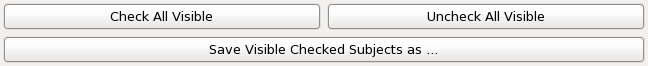
\includegraphics[width=1.0\textwidth,center]{saveSubjectList}
  				\caption{Save all sujects selected as one subject list}
    			\label{fig:saveSubjectList}
			\end{figure}
		\end{enumerate}
	\end{itemize}
	\subparagraph{\textbf{Note:}} Once you are done saving a subject list, you are asked if you want to use it right away for your study.
	\begin{figure}[H]
  		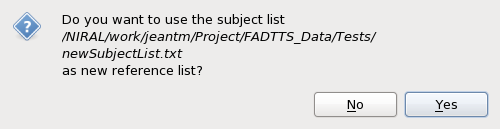
\includegraphics[width=0.6\textwidth,center]{useSavedSubjectList}
  		\caption{Use saved subject right away}
    	\label{fig:useSavedSubjectList}
	\end{figure}	
	\vfill
	\newpage
	
	\begin{itemize}
		\item \textbf{Search for subject(s):}
		\begin{itemize}
			\item Fill the search bar
		\end{itemize}
	\end{itemize}
	\begin{figure}[H]
		\makebox[\linewidth][c]{
			\centering
			\begin{subfigure}{0.75\textwidth}
        		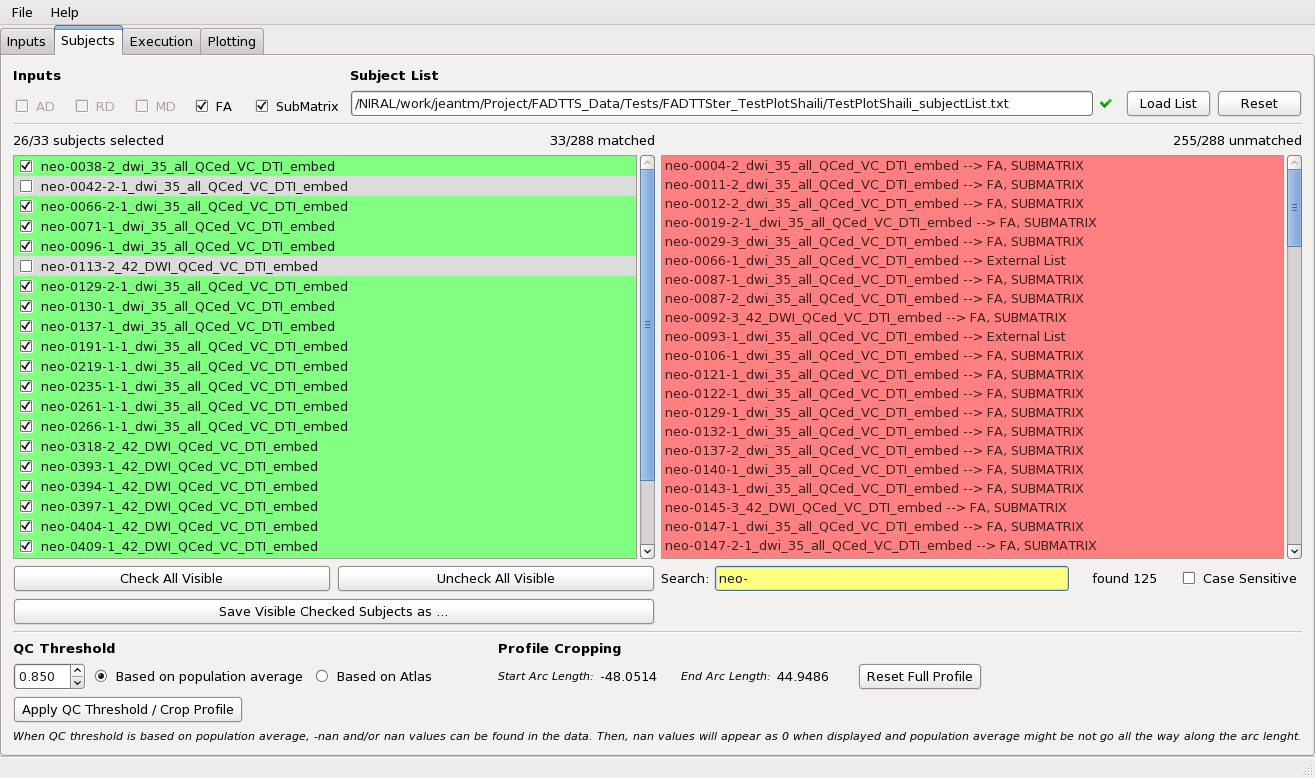
\includegraphics[width=\textwidth]{searchBefore}
        		\caption{Before}
        		\label{subfig:searchBefore}
    		\end{subfigure}
    		\begin{subfigure}{0.75\textwidth}
        		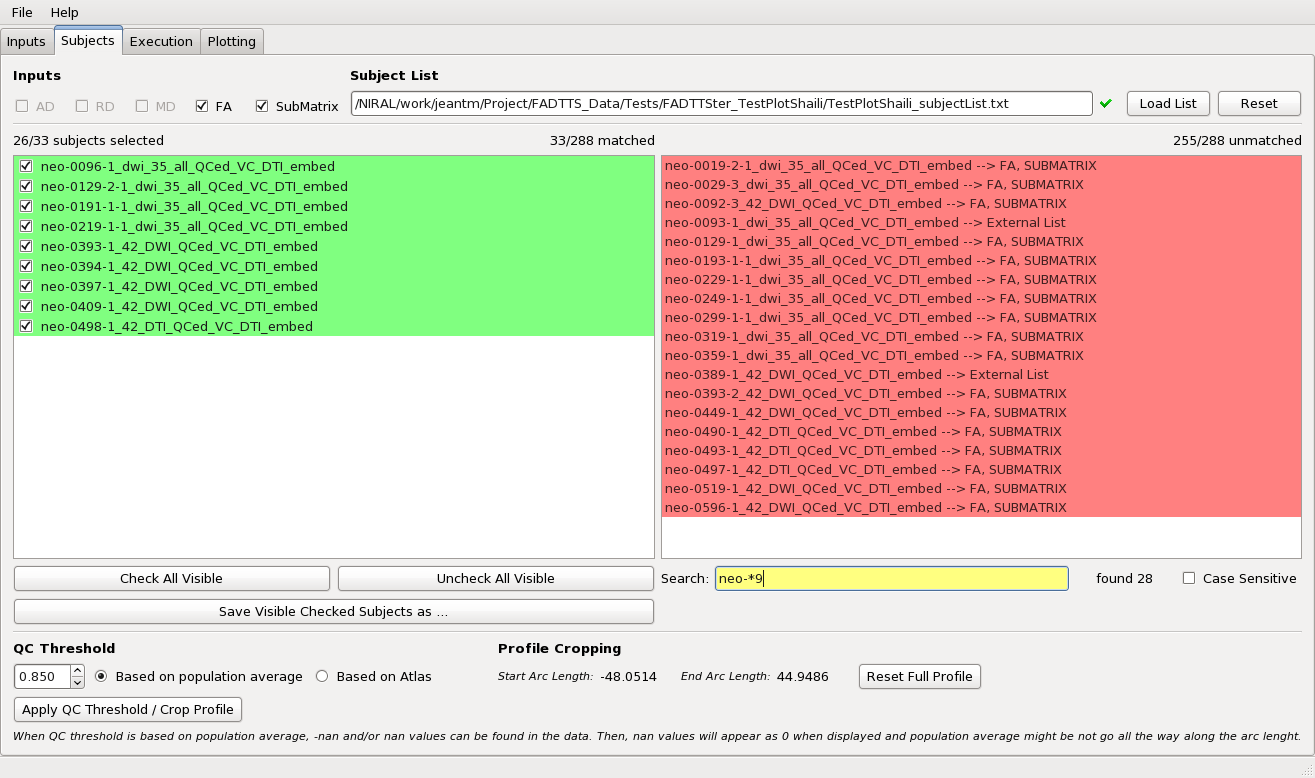
\includegraphics[width=\textwidth]{searchAfter}
        		\caption{After}
        		\label{subfig:searchAfter}
    		\end{subfigure}}
    	\caption{Searching for subjects}
    	\label{fig:SearchingSubjects}
	\end{figure}
	\subparagraph{\textbf{WARNING:}} A subject that does not fit the search remains checked as long as the user decides to modify its status. \textbf{Even if he is not displayed!}
	\subparagraph{\textbf{Note:}}
	\begin{itemize}
		\item[--] The search is done in both subjects' windows.
		\item[--] The character * replaces any sequence of characters.
		\item[--] As long as a seach is ongoing, the search bar remains highlighted in yellow.
	\end{itemize}
	\vfill
	\newpage
	
	\paragraph{Apply a QC threshold (FA file must be provided)}
	\begin{itemize}
		\item \textbf{Set QC threshold - \textit{Subjects} tab}
		\begin{enumerate}
			\item Set a value for the threshold (between 0 and 1)
			\item Choose on what the threshold base\newline (Atlas can only be chosen if it is provided in the last column of the FA file)
			\item Click on ``Apply QC Threshold / Crop Profile''
		\end{enumerate}
		\begin{figure}[H]
  			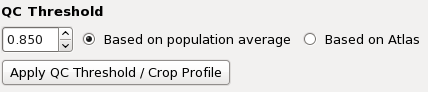
\includegraphics[width=0.75\textwidth,center]{applyQC0}
  			\caption{Setting the QC threshold in the \textit{Subjects} tab}
    		\label{fig:applyQC0}
		\end{figure}	
		\begin{figure}[H]
  			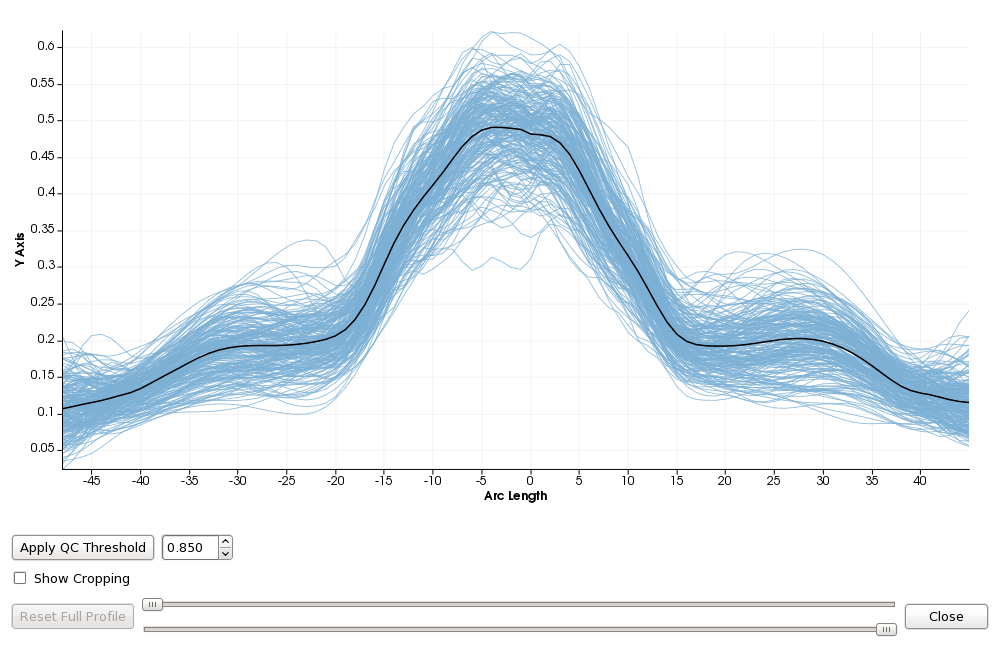
\includegraphics[width=1.0\textwidth,center]{applyQC1}
  			\caption{Pop-up window displayed to work on the QC threshold}
    		\label{fig:applyQC1}
		\end{figure}	
	\end{itemize}
	\vfill
	\newpage
	
	\begin{itemize}
		\item \textbf{Adjust QC threshold - pop-up window}
		\begin{enumerate}
			\item Adjust the QC threshold (value between 0 and 1)
			\item See which subjects will be removed from the study
		\end{enumerate}
		\begin{figure}[H]
  			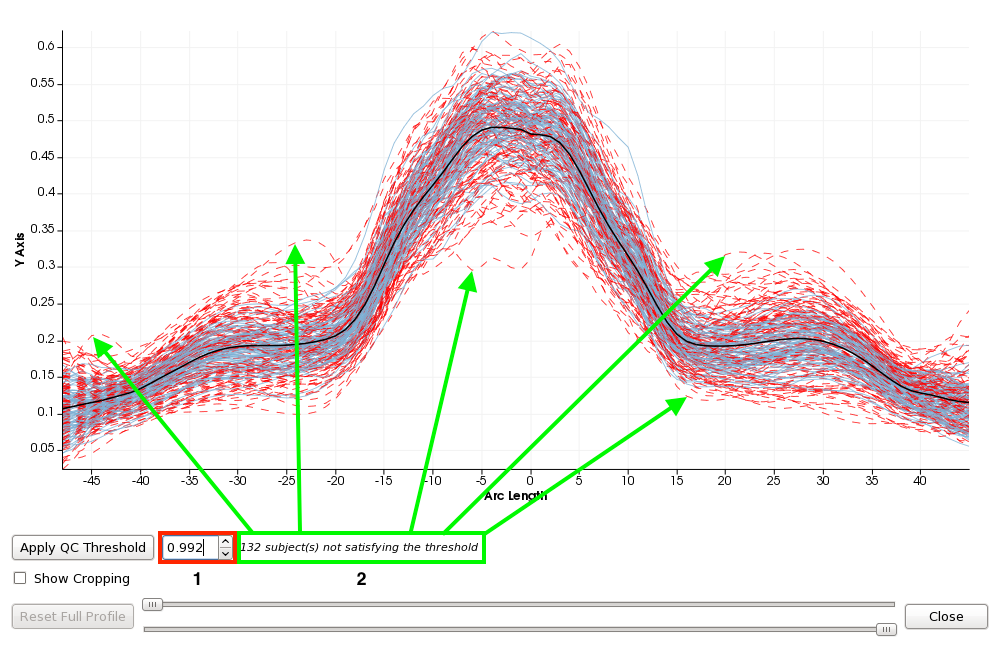
\includegraphics[width=0.9\textwidth,center]{applyQC2}
  			\caption{Adjusting the QC threshold}
    		\label{fig:applyQC2}
		\end{figure}
	\end{itemize}
	\begin{itemize}
		\item \textbf{Apply QC threshold}
		\begin{itemize}
			\item Click on ``Apply QC Threshold''
		\end{itemize}
	\end{itemize}
	\begin{figure}[H]
		\makebox[\linewidth][c]{
			\centering
			\begin{subfigure}{0.75\textwidth}
       			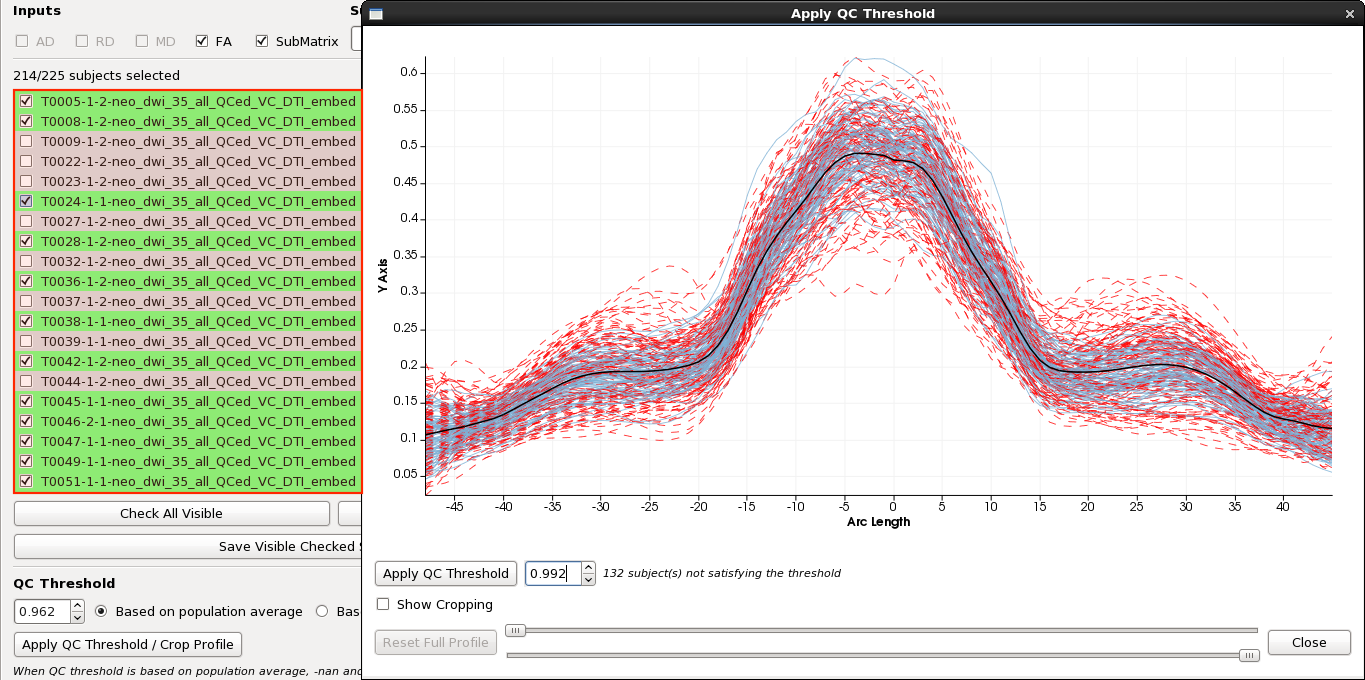
\includegraphics[width=\textwidth]{applyQC3}
       			\caption{Before}
       			\label{subfig:applyQC3}
    		\end{subfigure}
    		\begin{subfigure}{0.75\textwidth}
       			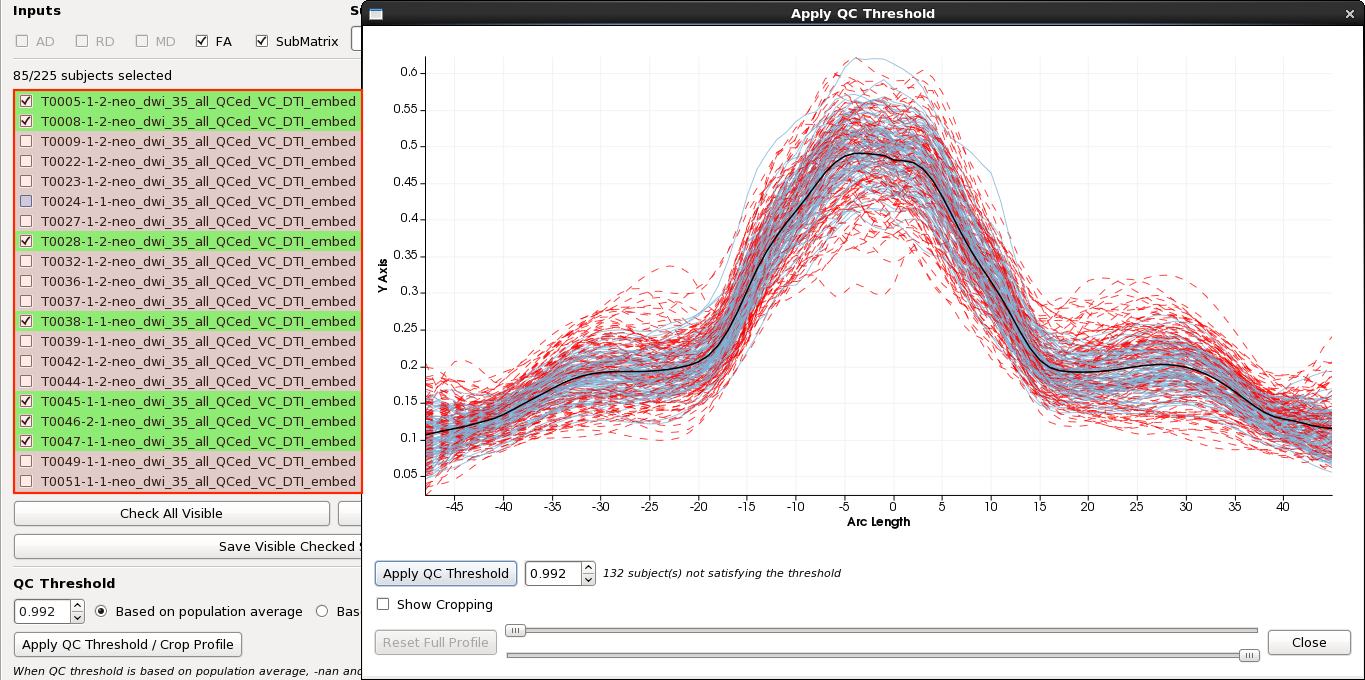
\includegraphics[width=\textwidth]{applyQC4}
       			\caption{After}
       			\label{subfig:applyQC4}
    		\end{subfigure}}
    	\caption{Apply a new QC threshold}
    	\label{fig:applyQCFinal}
	\end{figure}
	\subparagraph{\textbf{Note:}} Applying a QC threshold results in unchecking all subjects that do not satisfy that QC threshold.
	\vfill
	\newpage
	
	\paragraph{Crop profile (FA file must be provided)}
	\begin{enumerate}
		\item Click on ``Apply QC Threshold / Crop Profile''
		\item Set range of study using the two sliding bars
		\begin{figure}[H]
  			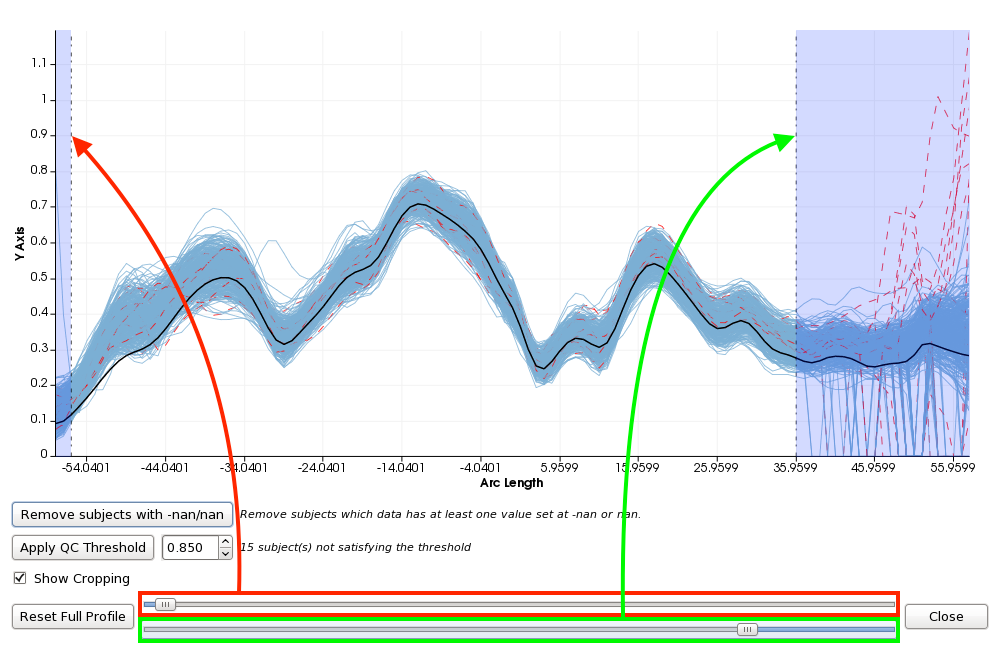
\includegraphics[width=0.84\textwidth,center]{profileCropping}
  			\caption{Adjusting the range of the study (highlighted zone are excluded)}
    		\label{fig:profileCropping}
		\end{figure}	
	\end{enumerate}
	\paragraph{Remove subjects with \textit{nan} values (FA file must be provided)}
	\begin{enumerate}
		\item Click on ``Apply QC Threshold / Crop Profile''
		\item If \textit{nan} values are found, click on ``Remove subjects with -nan/nan values''
	\end{enumerate}
	\begin{figure}[H]
		\makebox[\linewidth][c]{
			\centering
			\begin{subfigure}{0.65\textwidth}
       			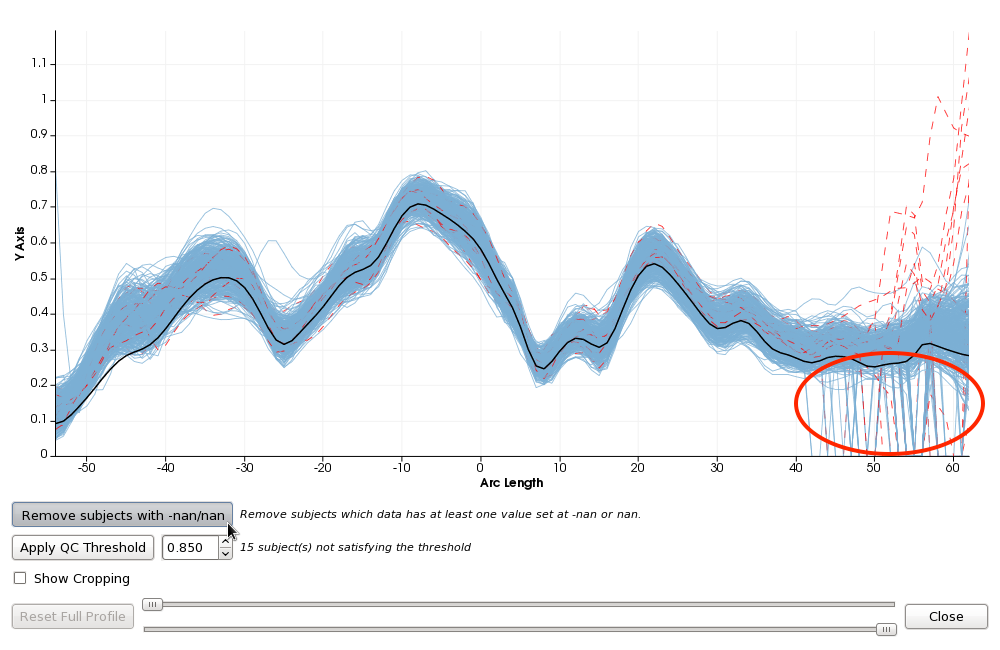
\includegraphics[width=\textwidth]{removeNANBefore}
       			\caption{Before}
       			\label{subfig:removeNANBefore}
    		\end{subfigure}
    		\begin{subfigure}{0.65\textwidth}
       			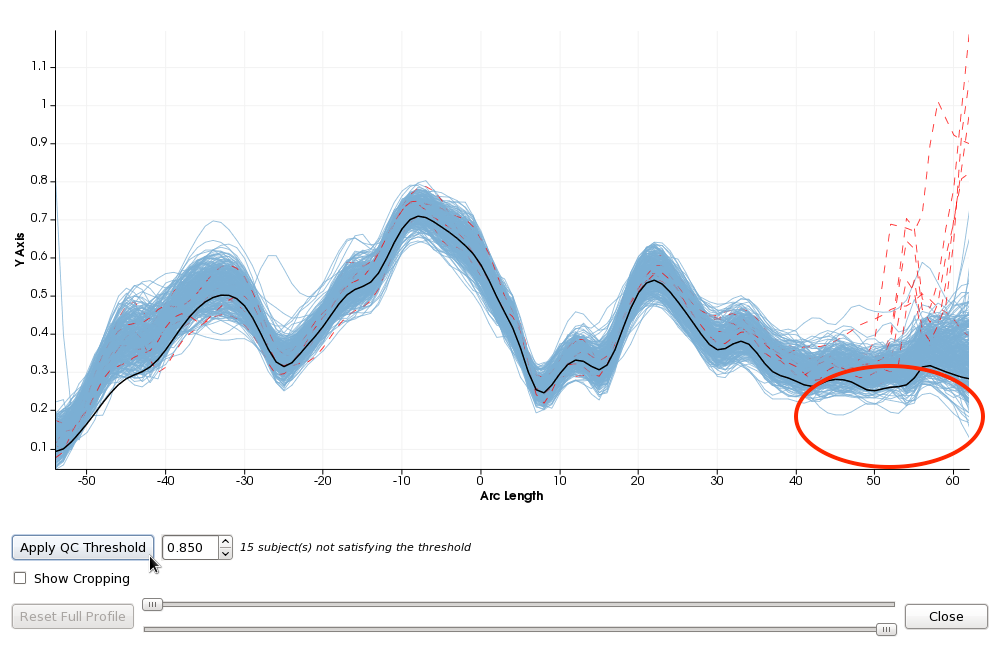
\includegraphics[width=\textwidth]{removeNANAfter}
       			\caption{After}
       			\label{subfig:removeNANAfter}
    		\end{subfigure}}
    	\caption{Removing \textit{nan} values}
    	\label{fig:removeNAN}
	\end{figure}	
	\vfill
	\newpage
	
	
	\subsubsection{Execution tab}
	\begin{figure}[H]
  		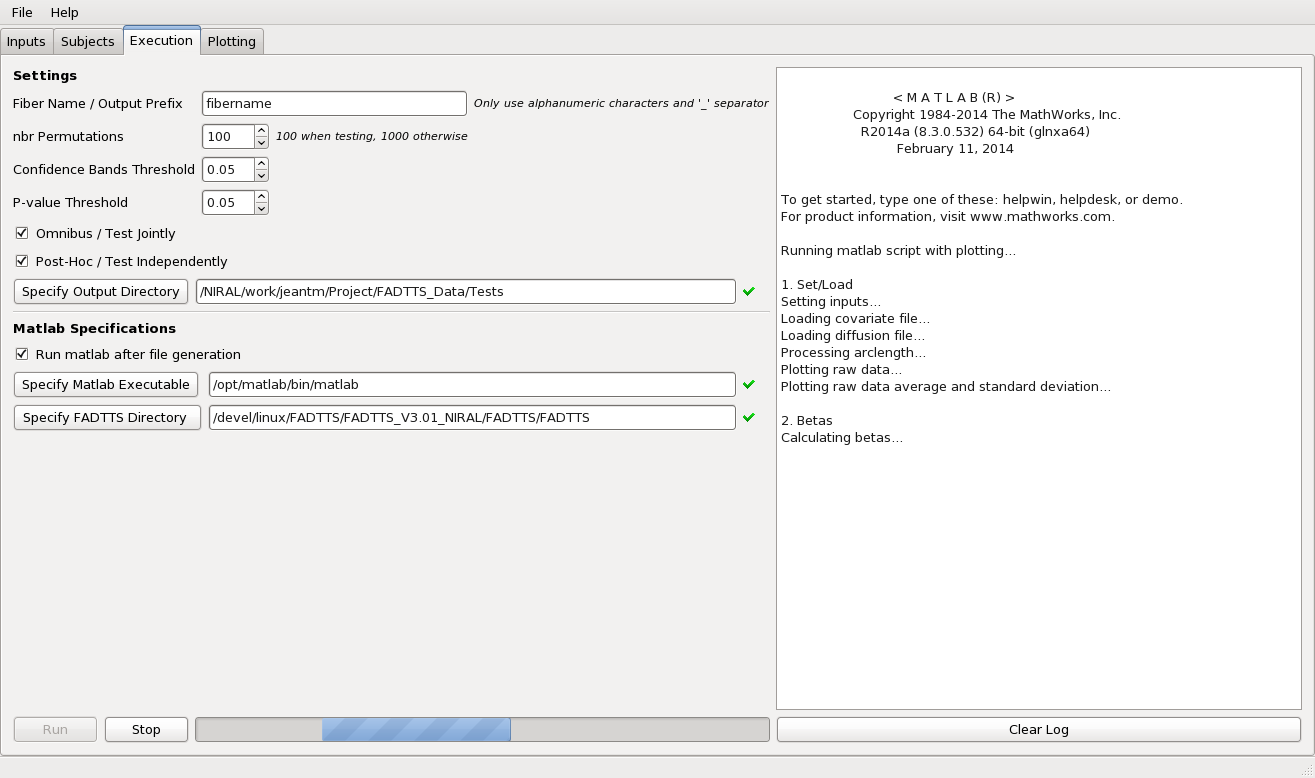
\includegraphics[width=1.36\textwidth,center]{runFADTTSter}
  		\caption{Execution tab}
    	\label{fig:runFADTTSter}
	\end{figure}
	The \textit{Execution} tab is where the user specifies the last information needed to run the \emph{Matlab script generation} such as the fiber name, the number of permutations, the confidence bands threshold, the FADTTS directory (where the Matlab FADTTS function are defined on the system or killDevil), etc.
	\vfill
	\newpage
	
	\paragraph{Adjuste settings and Matalb specifications}
	\begin{itemize}
		\item[--] Fiber name (Only use alphanumeric characters and ``\_'' separator!)
		\item[--] Number of permutations (value between 10 and 2000, usually 100 when testing, 1000 otherwise)
		\item[--] Confidence band Threshold (value between 0 and 1)
		\item[--] p-values threshold (value between 0 and 1)
		\item[--] Omnibus
		\item[--] Post-Hoc		
		\item[--] Output directory
	\end{itemize}
		
	\paragraph{Launch Matlab script generation}
	\begin{enumerate}
		\item Set FADTTS directory		
		\item If ``Run Matlab after file generation" is checked, set a Matlab executable
		\item Click on ``Run''
	\end{enumerate}
	\subparagraph{\textbf{WARNING:}}
	\begin{itemize}
		\item[--] Matlab R2013b or later is needed to run the script!
		\item[--] The computation of the script can be very long and use most of your computing power. We highly recommend that you launch your study on a remote server such as KillDevil instead of on your lab computer.
	\end{itemize}
	\subparagraph{\textbf{Note:}}
	\begin{itemize}
		\item[--] You can follow the script computation in real time in the log window.
		\item[--] Every file useful for the study is generated in the \textit{Output directory} specified by the user. New input files are generated based on the quality control of subjects and fibers.
	\end{itemize}
	\vfill
	\newpage
	
	\paragraph{Generated files}
	Every time FADTTSter is launched, a folder is created in the output directory provided. Its name is FADTTSter\_\textit{fibername}. All FADTTSter files are generated in this folder. After running FADTTSter, the following files are created:
	\begin{itemize}
		\item[--] FADTTSterAnalysis\_textit{fibername}\_\textit{nbrPermutations}perm.m\\
		Matlab script for the FADTTS computation.
		\item[--] myFDR.m\\
		Matlab function used in the Matlab script.
		\item[--] \textit{fibername}\_RawData\_\textit{property}.csv\\
		One for each property used for the study (\textit{AD}, \textit{RD}, \textit{MD}, \textit{FA}).\\
		Updated and cleaned version of the input property.
		\item[--] textit{fibername}\_RawData\_SUBMATRIX.csv\\
		Updated and cleaned version of the input property.
		\item[--] \textit{fibername}\_subjectList.txt\\
		List of all the subjects kept for the study.
		\item[--] \textit{fibername}\_subjectList\_NAN.txt\\
		List of all the subjects removed for the study because they contained at least one \textit{nan} value.
		\item[--] \textit{fibername}\_subjectList\_FAILED\_QCThreshold.txt\\
		List of all the subjects removed for the study because they failed the QC threshold.
		\item[--] configuration\_noGUI\_\textit{fibername}.json\\
		noGUI configuration file.
		\item[--] configuration\_softI\_\textit{fibername}.json\\
		Soft configuration file.
		\item[--] configuration\_para\_\textit{fibername}.json\\
		Parameters configuration file.
		\item[--] \textit{fibername}.log\\
		Log file containing all the information concerning the study.
	\end{itemize}
	\vfill
	\newpage
	
	In addition, if you have decided to run the script once it has been generated, a folder named MatlabOutputs is created. And, in this folder, you have the following files:
	\begin{itemize}
		\item[--] \textit{fibername}\_Betas\_\textit{property}.csv\\
		One for each property used for the study (\textit{AD}, \textit{RD}, \textit{MD}, \textit{FA}).
		\item[--] \textit{fibername}\_Omnibus\_Local\_pvalues.csv
		\item[--] \textit{fibername}\_Omnibus\_Global\_pvalues.csv
		\item[--] \textit{fibername}\_Omnibus\_FDR\_Local\_pvalues.csv
		\item[--] \textit{fibername}\_Omnibus\_ConfidenceBands\_\textit{property}.csv\\
		One for each property used for the study (\textit{AD}, \textit{RD}, \textit{MD}, \textit{FA}).
		\item[--] \textit{fibername}\_PostHoc\_Local\_pvalues\_\textit{property}.csv\\
		One for each property used for the study (\textit{AD}, \textit{RD}, \textit{MD}, \textit{FA}).
		\item[--] \textit{fibername}\_PostHoc\_Global\_pvalues.csv
		\item[--] \textit{fibername}\_PostHoc\_FDR\_Local\_pvalues\_\textit{property}.csv\\
		One for each property used for the study (\textit{AD}, \textit{RD}, \textit{MD}, \textit{FA}).
		\item[--] All Matlab figures
	\end{itemize}
\end{document}
